\documentclass[9pt, table]{beamer}
  \usetheme[block=fill]{metropolis}  % https://github.com/matze/mtheme

\usepackage{amsmath}
\usepackage{amssymb}
\usepackage{mathtools}
\usepackage{xcolor}
\usepackage{csquotes}
\usepackage{url}

\title{Machine Learning}
\date{}
\author{Thorben Menne}

\newcommand{\deriv}[1]{\mathrm{d}#1}
\newcommand{\dderiv}[2]{\frac{\mathrm{d}#1}{\mathrm{d}#2}}
\newcommand{\del}[1]{\partial #1}
\newcommand{\ddel}[2]{\frac{\partial #1}{\partial #2}}

\newcommand{\tcw}[1]{\textcolor{white}{#1}}
\newcommand{\tcb}[1]{\textcolor{black}{#1}}
\newcommand{\ccw}{\cellcolor{white}}
\newcommand{\ccga}{\cellcolor{black!50}}
\newcommand{\ccgb}{\cellcolor{black!40}}
\newcommand{\ccgc}{\cellcolor{black!30}}
\newcommand{\ccb}{\cellcolor{black}}

% Buffer slides for subsections (tex.stackexchange.com/questions/117658)
\AtBeginSubsection[]{
  \begin{frame}
    \subsectionpage
  \end{frame}
}


% Main title, author etc. in header
\subtitle{Part II -- Machine Learning Basics\\\vspace*{1.5ex}
  \small \textbf{Goal:} Gain basic understanding on why we need machine learning, what the differences between the many algorithms is and get introduced to some popular approaches
}

\begin{document}
  % Input after \begin{document} needs mdframed, listings, xcolor package
  % Make code snippets dark with rounded mdframe
  \mdfsetup{%
    backgroundcolor=col_bg,
    roundcorner=5pt,
    innerleftmargin=2em,  % 1em is for numbers
    innerrightmargin=1em,
    innertopmargin=0ex,
    innerbottommargin=0ex,
    skipabove=0.5\baselineskip,
    skipbelow=0.5\baselineskip,
  }
  \lstset{
    language=Python,  % Standard language
    inputpath=snippets,  % Where to search for lstinputlisting files
    tabsize=4,
    showspaces=false,  % Show space hints
    showstringspaces=true,
    numbers=left,  % Line numbering
    numbersep=1em,
  }
  \lstdefinestyle{dark}{%
    title=\lsttitledark{\lstname},
    basicstyle=\color{col_fg}\footnotesize\ttfamily,
    numberstyle=\color{col_fg}\tiny,
    commentstyle=\color{col_comment},
    % identifierstyle=\color{col_identifier},  % Not defined for Python
    keywordstyle=\color{col_keyword}\bfseries,
    stringstyle=\color{col_string},
    backgroundcolor=\color{col_bg},
    emph={range, enumerate},  % Additional coloring for given keywords
    emphstyle=\color{col_emph},
  }
  \lstdefinestyle{plain}{%
    numbers=none,
    basicstyle=\footnotesize\ttfamily,
    numberstyle=\tiny,
  }
  \maketitle

% %%%%%%%%%%%%%%%%%%%%%%%%%%%%%%%%%%%%%%%%%%%%%%%%%%%%%%%%%%%%%%%%%%%%%%%%%%%%%
% Intro
% %%%%%%%%%%%%%%%%%%%%%%%%%%%%%%%%%%%%%%%%%%%%%%%%%%%%%%%%%%%%%%%%%%%%%%%%%%%%%
\section{Introduction}

  \begin{frame}{Fitting a line to data}
    \begin{columns}
      \begin{column}{0.5\textwidth}
        \begin{itemize}
          \item One of the most basic but also often needed questions: I have some data points, which line fits them best?
          \item This is a classical supervised regression learning algorithm (although it's usually not called this way)
          \item Can be solved using maximum likelihood parameter estimation
          \begin{itemize}
            \item In case you think more of least squares: LSQ can be obtained as a special case of likelihood fitting using a Gaussian model for the data points
          \end{itemize}
          \item An analytic solution exist for this exact problem by maximizing
          \begin{equation*}
            \argmax_{\theta}\mathcal{L} \propto \prod_i
              \frac{1}{\sqrt{2\pi}\sigma}
              \exp{-\frac{(y_i - f(x_i|\theta))^2}{2\sigma^2}}
          \end{equation*}
          where the parameters only appear linear in $f$
        \end{itemize}
      \end{column}

      \begin{column}{0.5\textwidth}
        \includegraphics[width=\textwidth]{02-img-fit_straight_line_example}
      \end{column}

    \end{columns}
  \end{frame}

  \begin{frame}{Maximum Likelihood estimation}
    \begin{itemize}
      \item In general the idea of maximum Likelihood estimation (MLE) is to tune the model parameters so that the data appears to be most likely to originate from the tuned model
      \item This is expressed by maximizing the expression
        \begin{equation*}
          \mathcal{L}(x|\theta) = \prod_{i=1}^N f(x_i | \theta)
        \end{equation*}
        which is just the product of the PDF value for each of the $i=1, \dots, N$ data points $x_i$.
      \item For numerical reasons, almost always the negative log-Likelihood is minimized instead
      \begin{equation}
        -\ln\mathcal{L}(x\theta) = -\sum_{i=1}^N \ln(f(x_i | \theta))
      \end{equation}
      \item Some simple LLH parameter estimates can be derived analytically, like the straight line fit before, most are too complicated and require numerical solutions
      \item Note: The model selection is crucial in MLE, it incorporates all the knowledge we have of the estimated process, for example physical conditions
      \item Depending on the model, MLE can be used for regression as well as classification tasks
    \end{itemize}
  \end{frame}

  \begin{frame}{Maximum Likelihood example plot}
    \includegraphics[width=\textwidth]{02-img-likelihood_estimation_example}
  \end{frame}

  \begin{frame}{Logistic Regression}
    \begin{columns}
      \begin{column}{0.65\textwidth}
        \begin{itemize}
          \item In regression problems, like the line fit seen previously, it is tried to minimize the distance between the model and the data points
          \item However, in classification problems, data usually comes in discrete categories, also called classes
          \item These (binary) classes can be encoded with $Y\in {0, 1}$ (eg. sun will shine: $y=1$, sun won't shine: $y=0$), also called \enquote{one-hot-encoding}
          \item We can't simply fit a line to those data point, because the model would be meaningless
          \item The way around: Logistic Regression, which is, actually, a classification algorithm but uses regression to arrive there
          \item We use our Likelihood framework again, but we need to adapt our model to take the discrete classes into account
        \end{itemize}
      \end{column}
      \begin{column}{0.35\textwidth}
        \includegraphics[width=\textwidth]{02-img-logit}
      \end{column}
    \end{columns}
  \end{frame}

  \begin{frame}{Logistic Regression}
    \begin{columns}
      \begin{column}{0.65\textwidth}
        \begin{itemize}
          \item Using a modified Bernoulli LLH with a model of the success probability $p$ for a given $x_i$ rather than individual $p_i$ gives
          \begin{equation*}
            \mathcal{L} = \prod_i
              p(x_i | \theta)^{y_i} (1 − p(x_i | \theta))^{1 − y_i}
          \end{equation*}
          \item The most simple assumption for the model $p(x_i | \theta)$ is making it linear again, but now with a slight twist
          \begin{itemize}
            \item Because we want our model to predict between one and zero, not $p$ is assumed to be linear, but the expression $\ln{p / (1 - p)}$ (the \emph{logit} function)
            \item This seems arbitrary but, $p / (1 - p)$ are the odds and using the logarithm is a \enquote{natural} choice for extending the range to $[-\infty, \infty]$
          \end{itemize}
          \item We can then set
            \begin{equation}
              \ln \frac{p}{1 - p} = \theta x \Leftrightarrow
                p(x | \theta) = \frac{1}{1 + \exp(-\theta x)}
            \end{equation}
            which can be plugged into the Likelihood defined above
        \end{itemize}
      \end{column}
      \begin{column}{0.35\textwidth}
        \includegraphics[width=\textwidth]{02-img-logit}
      \end{column}
    \end{columns}
  \end{frame}

  \begin{frame}{Logistic Regression example plot}
    \includegraphics[width=\textwidth]{02-img-logistic_regression}
  \end{frame}

  \begin{frame}{Why do we need ML then?}
    \begin{columns}[c]
      \begin{column}{0.8\textwidth}
        \begin{itemize}
          \item With the maximum Likelihood formalism we have a very versatile and mighty tool at our hands
          \begin{itemize}
            \item It can be used to model regression and even classification tasks and estimate optimal parameters
            \item There is also a whole class of algorithms utilizing Bayes theorem to make posterior predictions (not covered here)
          \end{itemize}
          \item \textbf{So why do we need machine learning at all then?}
          \item For complex tasks, model building becomes equivalently complex
          \begin{itemize}
            \item How to write down a model for recognizing items in images?
              Potentially impossible to craft manually
            \item Model must be robust against rotation, translation, scaling, color variations, lightning variations, variations in the item itself, etc, etc ...
          \end{itemize}
          \item Big advantage of machine learning, aka the \enquote{learning}: Using an algorithm that \enquote{learns} the model itself by some kind of predefined measure (aka loss function) from a given dataset representing examples from the target distribution
          \begin{itemize}
            % \item Note: The term \enquote{learning} should not be understood to mean the same as human learning generally means.
            \item In general, the models are so general, that they adapt to many problems with very good performance
            \item In the end, it's \emph{just curve fitting}
          \end{itemize}
        \end{itemize}
      \end{column}
      \begin{column}{0.2\textwidth}
        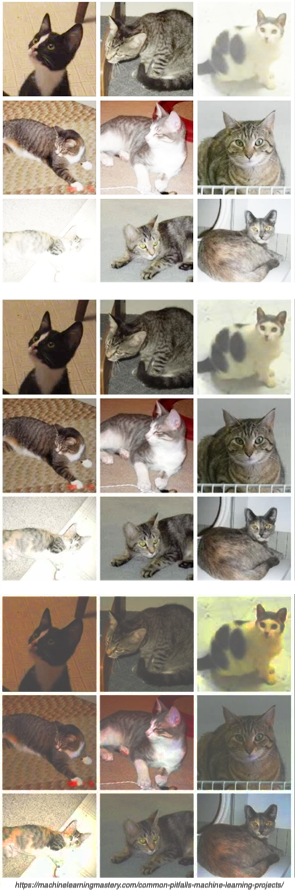
\includegraphics[height=0.9\textheight]{02-img_cat_examples}
      \end{column}
    \end{columns}
  \end{frame}

  \begin{frame}{Different tasks to solve with ML}
    Different task in which machine learning algorithms are used (not complete):
    \begin{description}
      \item [Classic classification] Sorting inputs in previously specified $k$ classes.
        Typically resembles a function $\mathbb{R}^n \rightarrow \{1, \dots, k\}$
      \item [Classic regression] The other classical task, predicting a continuous value from the input, typically $\mathbb{R}^n \rightarrow \mathbb{R}$
      \item [Transcription] Converting some kind of rather unstructured input (voice, text in image, etc.) in textual form (heavily used in modern speech recognition)
      \item [Translation] Translating between languages.
        Set in the field of natural language processing.
      \item [Anomaly detection] Noticing any kind of unusual behaviour or outliers in input data
      \item [Synthesis] Generating new data that looks similar to previously shown data.
        Eg. \emph{Deep Fake} or speech synthesis.
      \item [Filling of missing values] Filling \enquote{holes} in input data.
        Can be used to patch images with missing data or similar tasks
      \item [Denoising] Reducing noise in input data, for example in super resolution or also speech recognition
    \end{description}
  \end{frame}

  \begin{frame}{Performance measure}
    \begin{columns}
      \begin{column}{0.65\textwidth}
        \begin{itemize}
          \item In machine learning algorithms, the definition of the loss function is the key task to define the behaviour and the capabilities of the learned system
          \item Defining the loss can get quite complicated to find the desired result
          \item For classification tasks, usually a simple \emph{accuracy} measure is used, which is just the proportion of correctly classified samples and usually encoded using the \emph{cross-entropy loss}
          \item For regression tasks, the mean squared error is often used to measure the deviation of the model output to the data point for each sample.
            Many variants exists, for example for regularization (Huber loss)
          \item For example in a style transfer generative model, the loss is a combination from a \emph{style loss} and \emph{content loss} to produce the desired output.
        \end{itemize}
      \end{column}
      \begin{column}{0.35\textwidth}
        \vspace*{1em}
        \includegraphics[width=\textwidth]{02-img-loss_functions}
      \end{column}
    \end{columns}
  \end{frame}

  \begin{frame}{Supervised / unsupervised learners}
    \begin{columns}[t]
      \begin{column}{0.65\textwidth}
        \begin{itemize}
          % \item Machine learning algorithms can roughly be separated into \emph{supervised} and \emph{unsupervised} algorithms
          \item \textbf{Supervised algorithms} are given a training data set with known labels
          \begin{itemize}
            \item In each learning step, the algorithm can compare its results to the ground truth, adapt and get better over time
            \item Popular example algorithms are: Naive Bayes, k-nearest neighbour, support vector machines, tree based learners, Neural Networks, linear discriminants and again linear regression
          \end{itemize}
          \item \textbf{Unsupervised algorithms} aim to work on datasets with no class information available  % and try to reduce the need for human oversight to a minimum
          \begin{itemize}
            \item Not being able to learn from a ground truth, such models usually try to find a representation of the underlying data distribution.
            \item Clustering algorithms, like k-means, try to group data points based on some distance measure
              % Cross validation can be used to estimate hyper-parameters like the number of clusters to find
            \item Neural network autoencoders try to find a compressed version of the input by piping the data through a bottleneck and then reconstructing them from that reduced input.
              % They can thus compare the input to their own generated output
            \item \emph{Expectation-maximization} is an iterative Likelihood method and is used in Gaussian mixture models
          \end{itemize}
          % \item Here focus mostly on an overview of supervised learners
        \end{itemize}
      \end{column}
      \begin{column}{0.35\textwidth}
        \vspace*{1em}
        \includegraphics[width=\textwidth]{02-img-supervised_unsupervised_comic}
      \end{column}
    \end{columns}
  \end{frame}

  \begin{frame}{Info graphic supervised}
      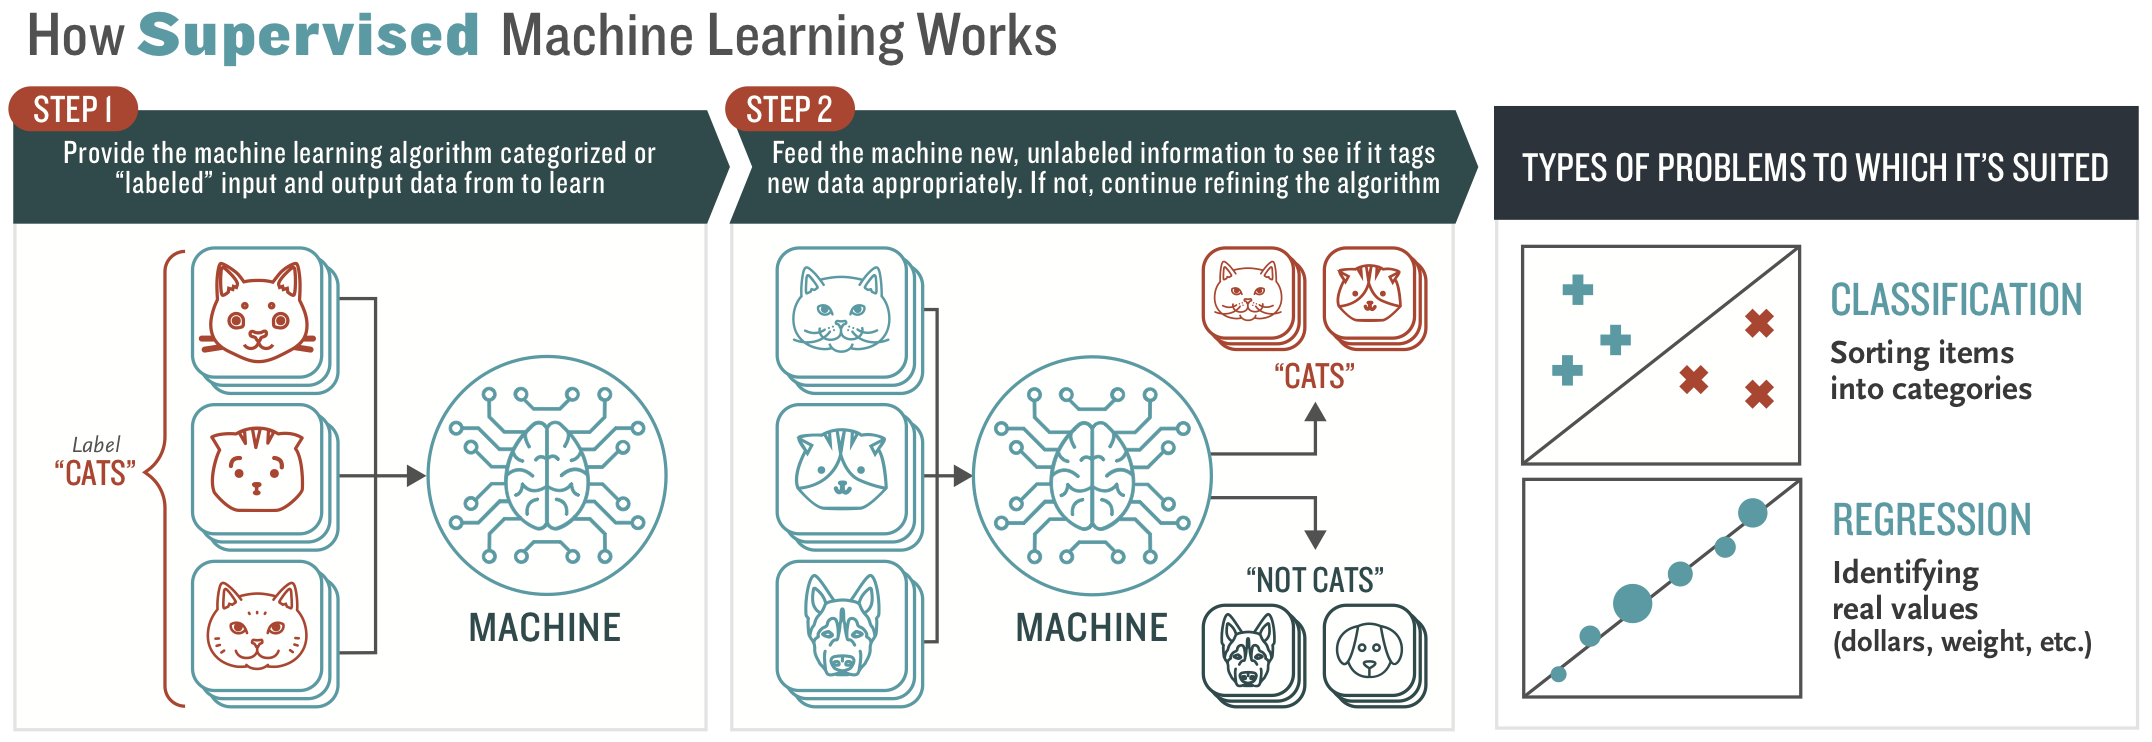
\includegraphics[width=\textwidth]{02-img-how-do-machines-learn_supervised}
      \begin{center}
        \tiny[\url{https://www.boozallen.com/content/dam/boozallen_site/sig/pdf/infographic/how-do-machines-learn.pdf}]
      \end{center}
  \end{frame}

  \begin{frame}{Info graphic unsupervised}
      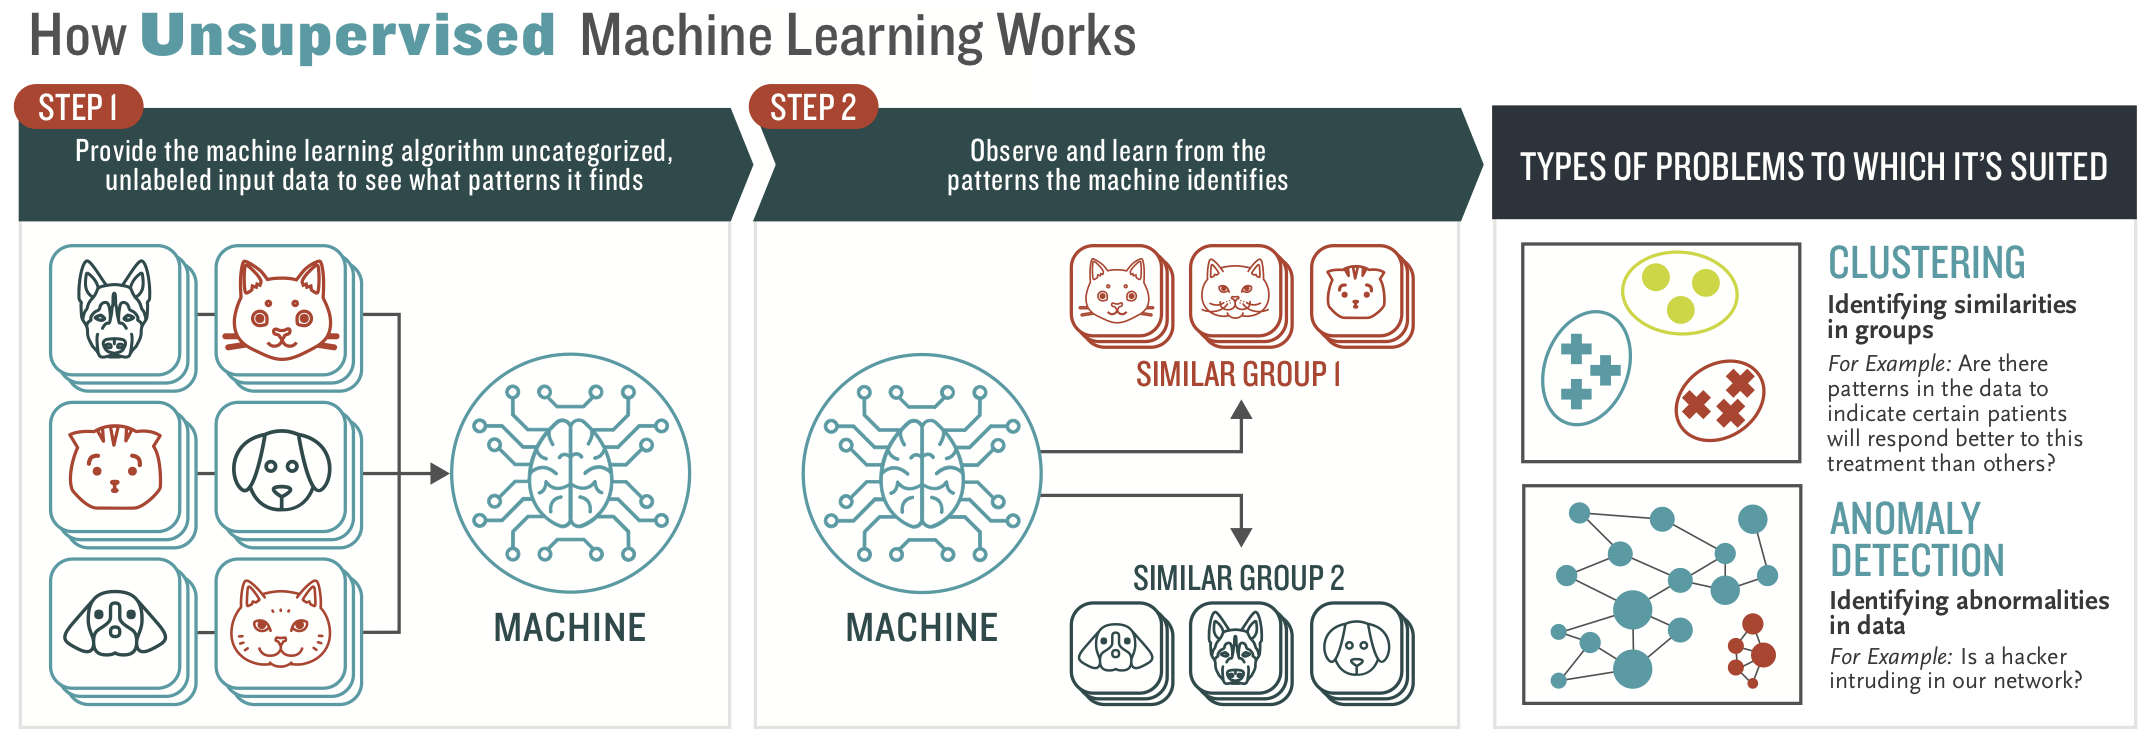
\includegraphics[width=\textwidth]{02-img-how-do-machines-learn_unsupervised}
      \begin{center}
        \tiny[\url{https://www.boozallen.com/content/dam/boozallen_site/sig/pdf/infographic/how-do-machines-learn.pdf}]
      \end{center}
  \end{frame}


% %%%%%%%%%%%%%%%%%%%%%%%%%%%%%%%%%%%%%%%%%%%%%%%%%%%%%%%%%%%%%%%%%%%%%%%%%%%%%
% Basics
% %%%%%%%%%%%%%%%%%%%%%%%%%%%%%%%%%%%%%%%%%%%%%%%%%%%%%%%%%%%%%%%%%%%%%%%%%%%%%
  \section{Basics}

    \begin{frame}{Overfitting / underfitting}
      \begin{itemize}
        \item A key challenge in machine learning applications is that the focus lies more on a broad validity of the model rather than trying to get the maximum information from the training set
        \item This means the trained model should also behave well on previously unseen data, not used in training
      \end{itemize}
    \end{frame}

    \begin{frame}{Validation}
      \begin{itemize}
        \item Validation in general
        \item Cross validation
      \end{itemize}
    \end{frame}

    \begin{frame}{Regularization}
      \begin{itemize}
        \item Underconstrained LinEqSys
        \item L2 Regularization example
        \item Examples in other contexts
      \end{itemize}
    \end{frame}

    \begin{frame}{Hyperparamter search / tuning}
      \begin{itemize}
        \item Grid search
        \item Random search
      \end{itemize}
    \end{frame}

    \begin{frame}{Variance Bias tradeoff}
      \begin{itemize}
        \item Tree pruning as example
      \end{itemize}
    \end{frame}

    \begin{frame}{Feature extraction / generation}
      \begin{itemize}
        \item PCA -> Also shortly mention as a unsupervised learner
        \item Generative algorithms
      \end{itemize}
    \end{frame}

    \begin{frame}{Feature selection}
      \begin{itemize}
        \item MRMR
        \item Forward / backward selection
      \end{itemize}
    \end{frame}

  \subsection{Regression}

  \begin{frame}{Intro}
    \begin{itemize}
      \item What is regression
      \item Loss function
      \item Example
    \end{itemize}
  \end{frame}

  \subsection{Classification}

  \begin{frame}{Intro}
    \begin{itemize}
      \item What is classification
      \item Loss function
      \item Example
    \end{itemize}
  \end{frame}

% %%%%%%%%%%%%%%%%%%%%%%%%%%%%%%%%%%%%%%%%%%%%%%%%%%%%%%%%%%%%%%%%%%%%%%%%%%%%%
% Example ALgoithms
% %%%%%%%%%%%%%%%%%%%%%%%%%%%%%%%%%%%%%%%%%%%%%%%%%%%%%%%%%%%%%%%%%%%%%%%%%%%%%
\section{Algorithms}
  \subsection{Supervised}

  \begin{frame}{Curve Fitting - Least Squares}
  Regression
  \end{frame}

  \begin{frame}{KNN Classification}
  Classification
  \end{frame}

  \begin{frame}{LDA Classification}
  Classification
  \end{frame}

  \begin{frame}{Support Vector Machine}
  Classification
  Regression
  \end{frame}

  \begin{frame}{Naive Bayes Classifier}
  Classification
  \end{frame}

  \begin{frame}{Tree Based Learners}
  Classification
  Regression
  \end{frame}

  \begin{frame}{Neural Networks}
  Classification
  Regression
  Only briefly
  \end{frame}

  \subsection{Unsupervised}

  \begin{frame}{Clustering}
  k-Means
  Mention DBSCAN
  \end{frame}

  \begin{frame}{Generative Neural Network Models}
  Mention GANs, Autoencoders
  \end{frame}



\end{document}
